%! Author = ASUS
%! Date = 7/2/2023

% Preamble
\documentclass[11pt]{article}

% Packages
\usepackage{amsmath}
\usepackage{lipsum}
\usepackage{wasysym}
\usepackage{subcaption}
\usepackage{adjustbox}
\usepackage{multirow}
\usepackage{graphicx}
\usepackage{float}
\usepackage{listings}
\usepackage{xcolor}
\usepackage{pgfplots}
% Document
\begin{document}
    We will explore the application of Structure from Motion in a real-world scenario within the field of 3D
    computer vision. Our goal is to localize a robot in a large city environment using point cloud registration.
    Localization refers to the task of determining the position and orientation of a robot within its environment.
    And, point cloud registration is defined as finding the transformation, i.e. translation and orientation,
    that aligns the points in one point cloud with those in another.

    Outdoor localization, today, relies heavily on GPS technology, accompanied by ground based augmentation systems
    to improve accuracy. However, in this thesis, we are going to explore a method that makes it offline, meaning
    eliminating the need for GPS or similar devices.

    \section{Point Cloud Generation}
    \subsection{Image Acquisition}
    A GoPro9 camera is mounted on the head of a vehicle, and various videos are taken from the streets.
    The videos were recorded at a frame rate of 60 fps. The resolution of each image is 1920*1080 pixels,
    and the distance covered in each video ranges from 80 to 120 meters. We used the linear settings for the camera,
    meaning that the camera undistorts the videos automatically. We also, tested with distorted settings and manual calibration
    (See \ref{calib_impact}). However, using undistorted videos showed better results. Next, the frames are extracted for each video.
    The rate of the sampling is chosen at 3fps. Each dataset comprises an average of 60 frames.

    \subsection{Reconstruction}
    Structure from Motion algorithm is used to reconstruct the 3D scene of the environment. There are 2 types of reconstruction:
    \begin{itemize}
        \item Sparse Reconstruction estimates the positions of a relatively small number of keypoints detected on the input images
        \item Dense Reconstruction provides 3D positions for all pixels in the input images by generating depth maps.
    \end{itemize}
    COLMAP is an open source software, implemented by ~\cite{schoenberger2016sfm} and ~\cite{schoenberger2016mvs},
    that provides 3D reconstruction based on 2D images. Spare and Dense Reconstructions are both implemented in COLMAP.
    Dense reconstruction is achievable after obtaining
    the sparse reconstruction with camera poses. By default, It runs PatchMatch algorithm \cite{journals/tog/BarnesSFG09} to extract dense point clouds.
    Each step of SfM pipline can be executed separately. So, other algorithm can be replaced by its defaults. And, extra steps, like refinements, can be added to the pipeline.


    Figure \ref{fig:sfm} shows examples of both reconstructions.
    For our method, we need dense point clouds.

    \begin{figure}
        \centering
        \begin{subfigure}{0.45\textwidth}
            \centering
            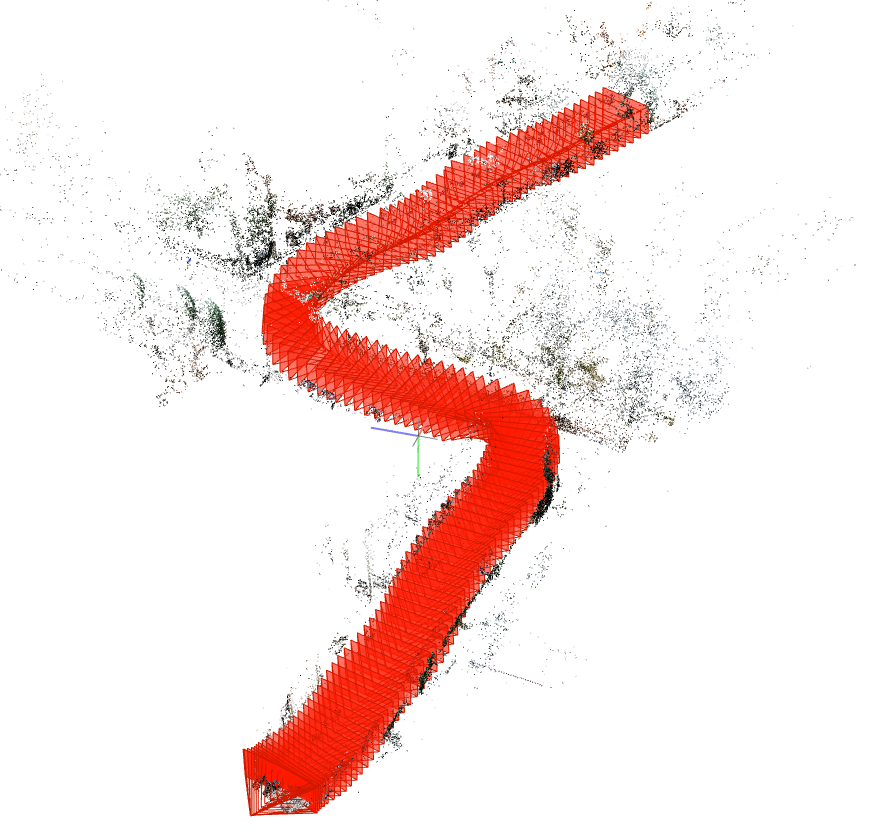
\includegraphics[width=\linewidth]{images/method/sfm_sparse_1}
            \caption{Example 1: Sparse Point cloud}
        \end{subfigure}
        \hfill
        \begin{subfigure}{0.45\textwidth}
            \centering
            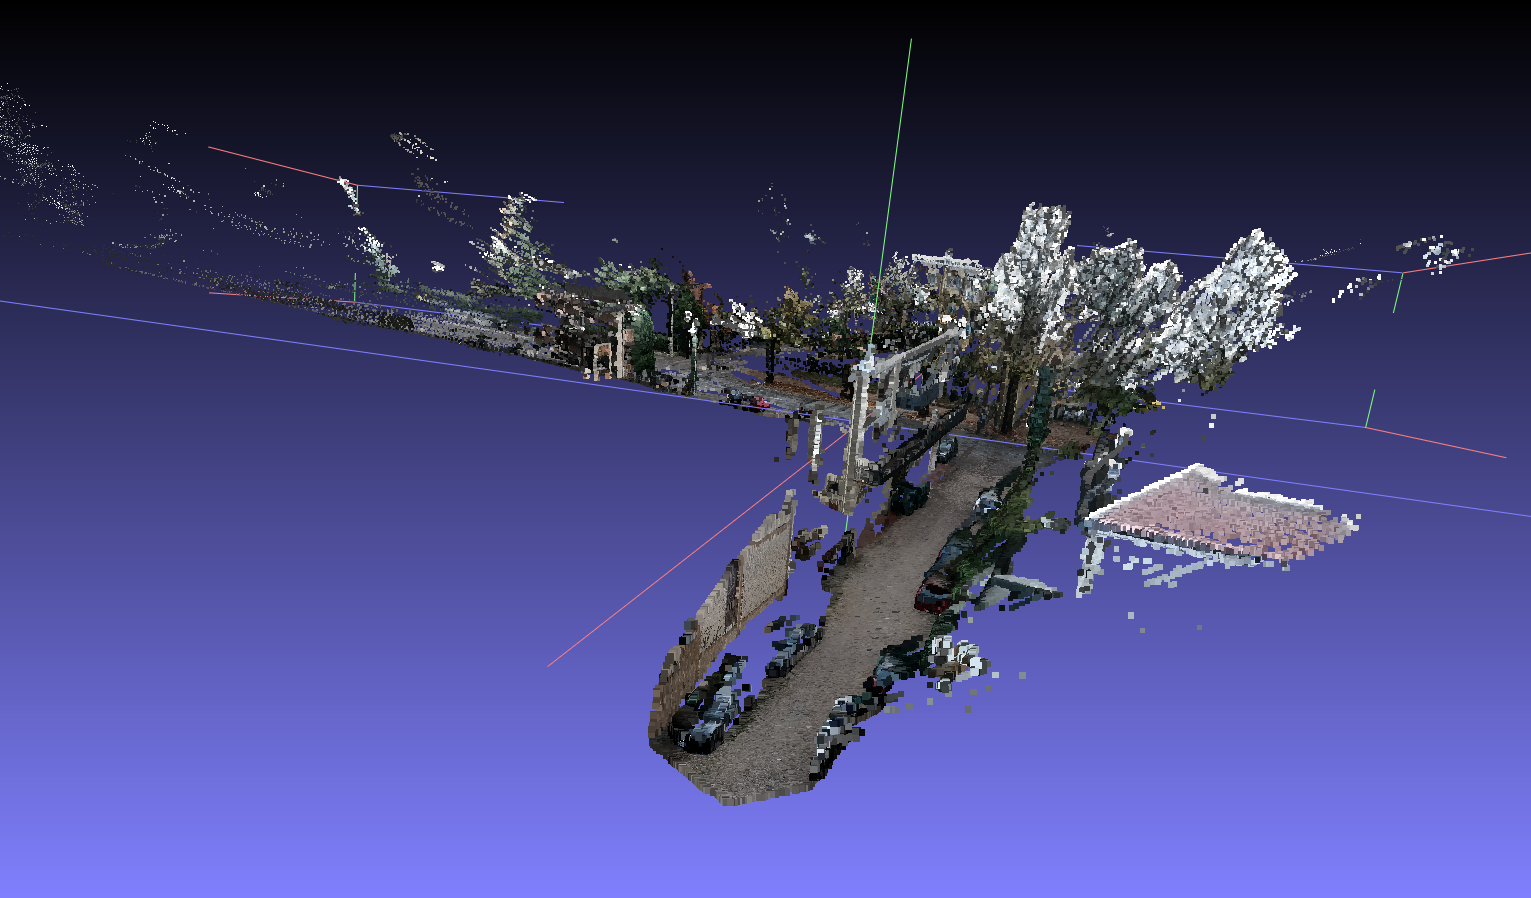
\includegraphics[width=\linewidth]{images/method/sfm_dense_1}
            \caption{Example 1: Dense Point cloud}
        \end{subfigure}

        \vspace{1em}

        \begin{subfigure}{0.45\textwidth}
            \centering
            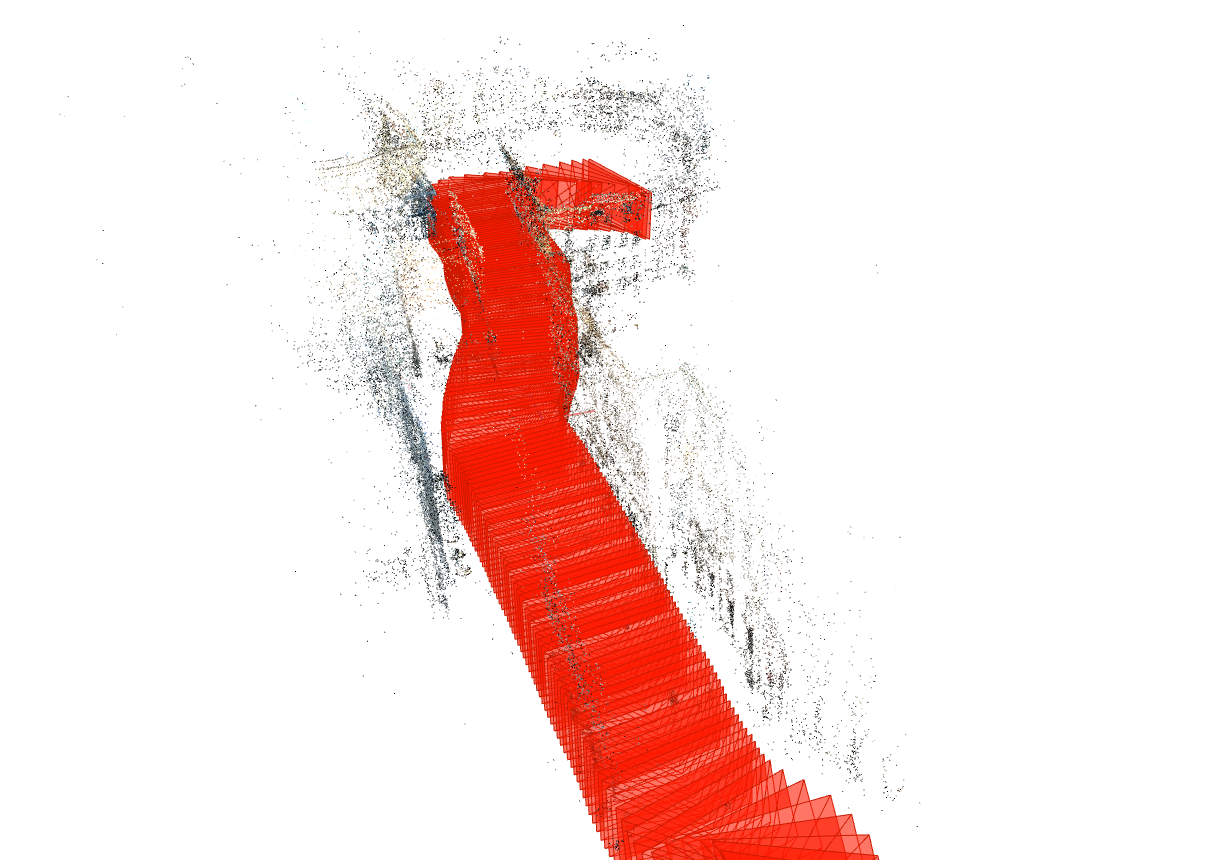
\includegraphics[width=\linewidth]{images/method/sfm_sparse_2}
            \caption{Example 2: Sparse Point cloud}
        \end{subfigure}
        \hfill
        \begin{subfigure}{0.45\textwidth}
            \centering
            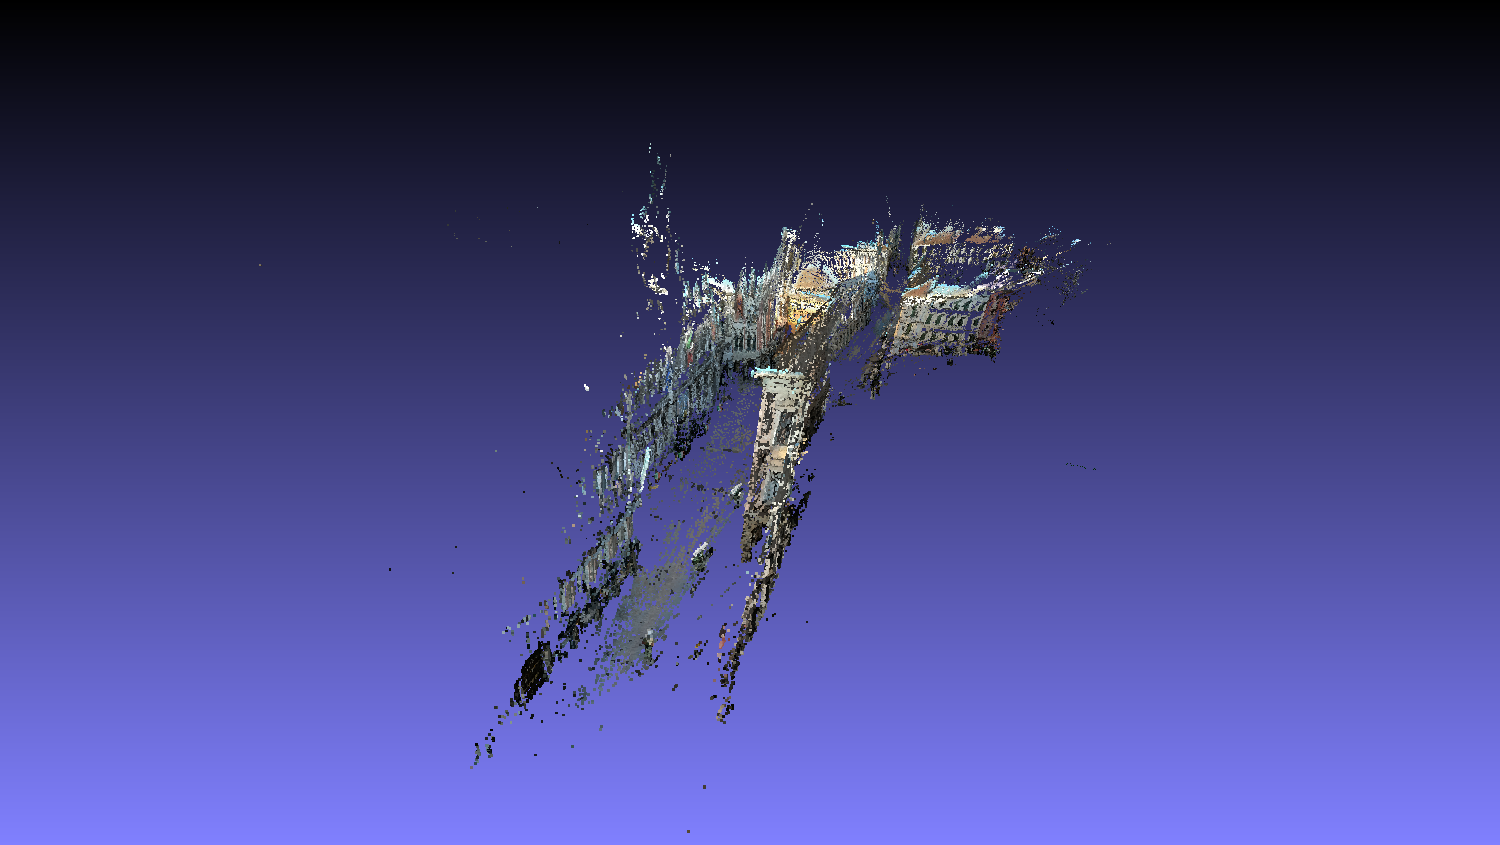
\includegraphics[width=\linewidth]{images/method/sfm_dense_2}
            \caption{Example 2: Dense Point cloud}
        \end{subfigure}

        \caption{Comparing sparse and dense reconstructions, generated by COLMAP ~\cite{schoenberger2016sfm} and ~\cite{schoenberger2016mvs}}
        \label{fig:sfm}
    \end{figure}

    \subsection{Refinement}
    Pixel-Perfect paper \cite{lindenberger2021pixsfm} is decided to be used for our reconstruction refinement.
    First, in order to verify that this paper can actually refine the reconstruction, a test dataset is
    created from a cereal box on a table, and dense 3D point cloud is obtained by COLMAP
    and refined by pixel perfect. In figure \ref{fig:cereal}, it can be clearly seen that their approach is improving the reconstruction.
    In our datasets, which contain points of street, and buildings, the refinement results in more 3D points of streets, figure \ref{fig:ref_sfm}.
    We will see later, that more coverage of the streets is crucial for our method of localization.
    In our method, first, the initial sparse point cloud and camera poses are generated by COLMAP. Then, they are refined
    by pixel-perfect algorithm. And after that, the dense construction is executed for each dataset.

    \begin{figure}
        \centering
        \begin{subfigure}{0.45\textwidth}
            \centering
            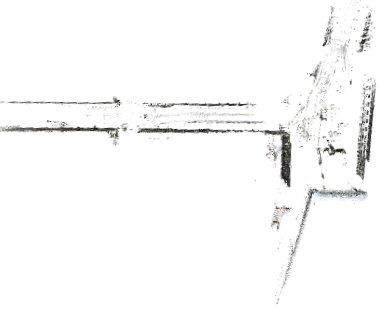
\includegraphics[width=\linewidth]{images/method/refine_before}
            \caption{Before Refinement}
        \end{subfigure}
        \hfill
        \begin{subfigure}{0.45\textwidth}
            \centering
            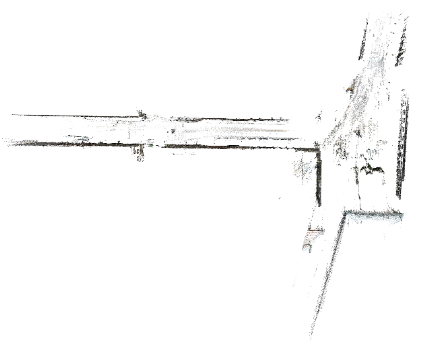
\includegraphics[width=\linewidth]{images/method/refine_after}
            \caption{After Refinement}
        \end{subfigure}
        \caption{Sparse reconstruction refinement using Pixel-Perfect paper, \cite{lindenberger2021pixsfm}}
        \label{fig:ref_sfm}
    \end{figure}

    \begin{figure}
    \centering
    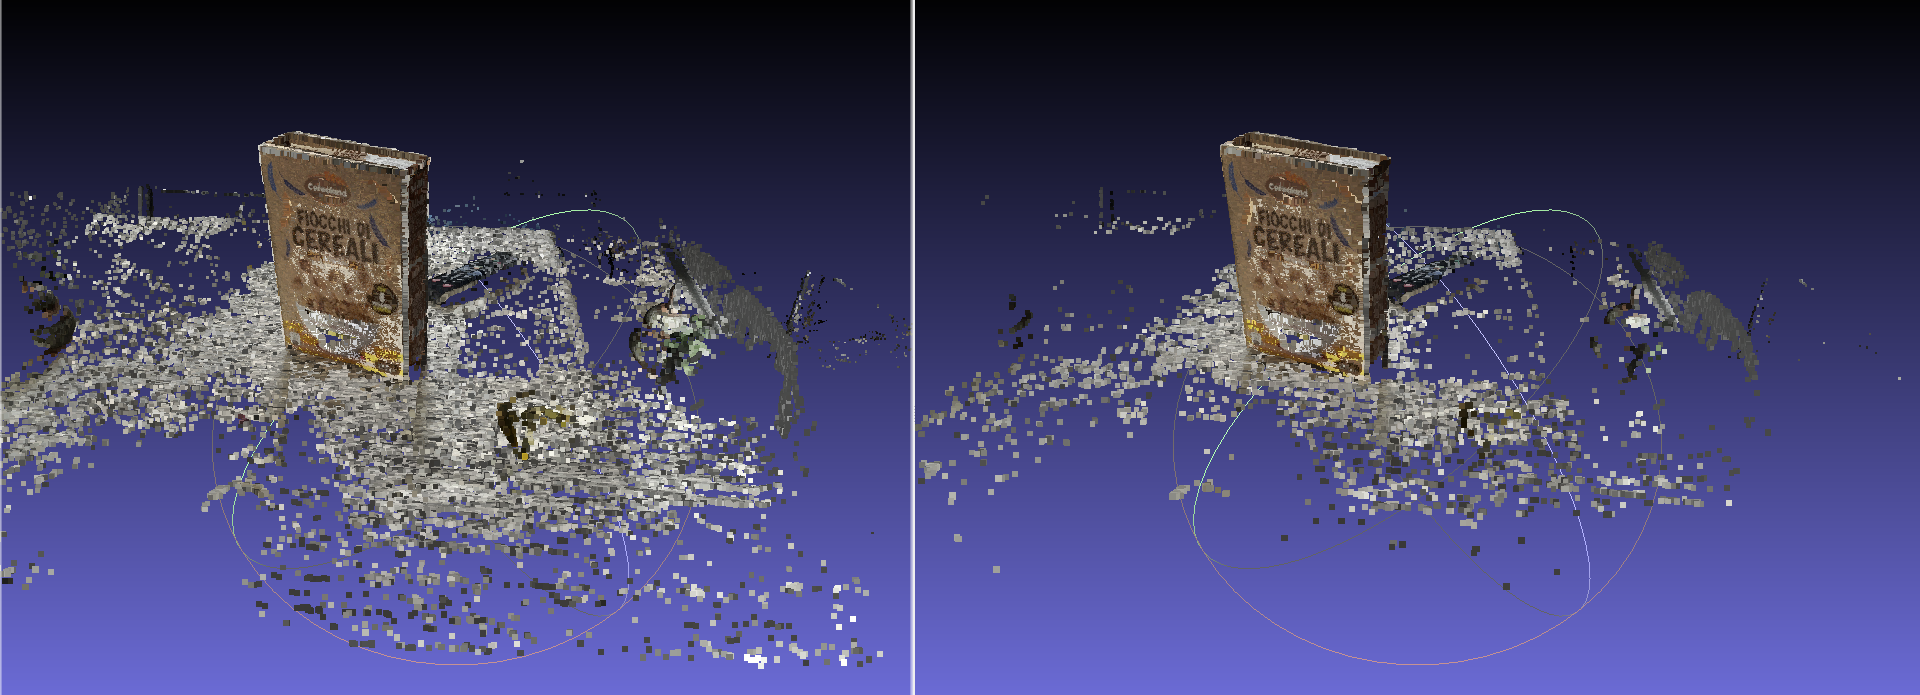
\includegraphics[width=\textwidth,height=\textheight,keepaspectratio]{images/cereal.1.png}
    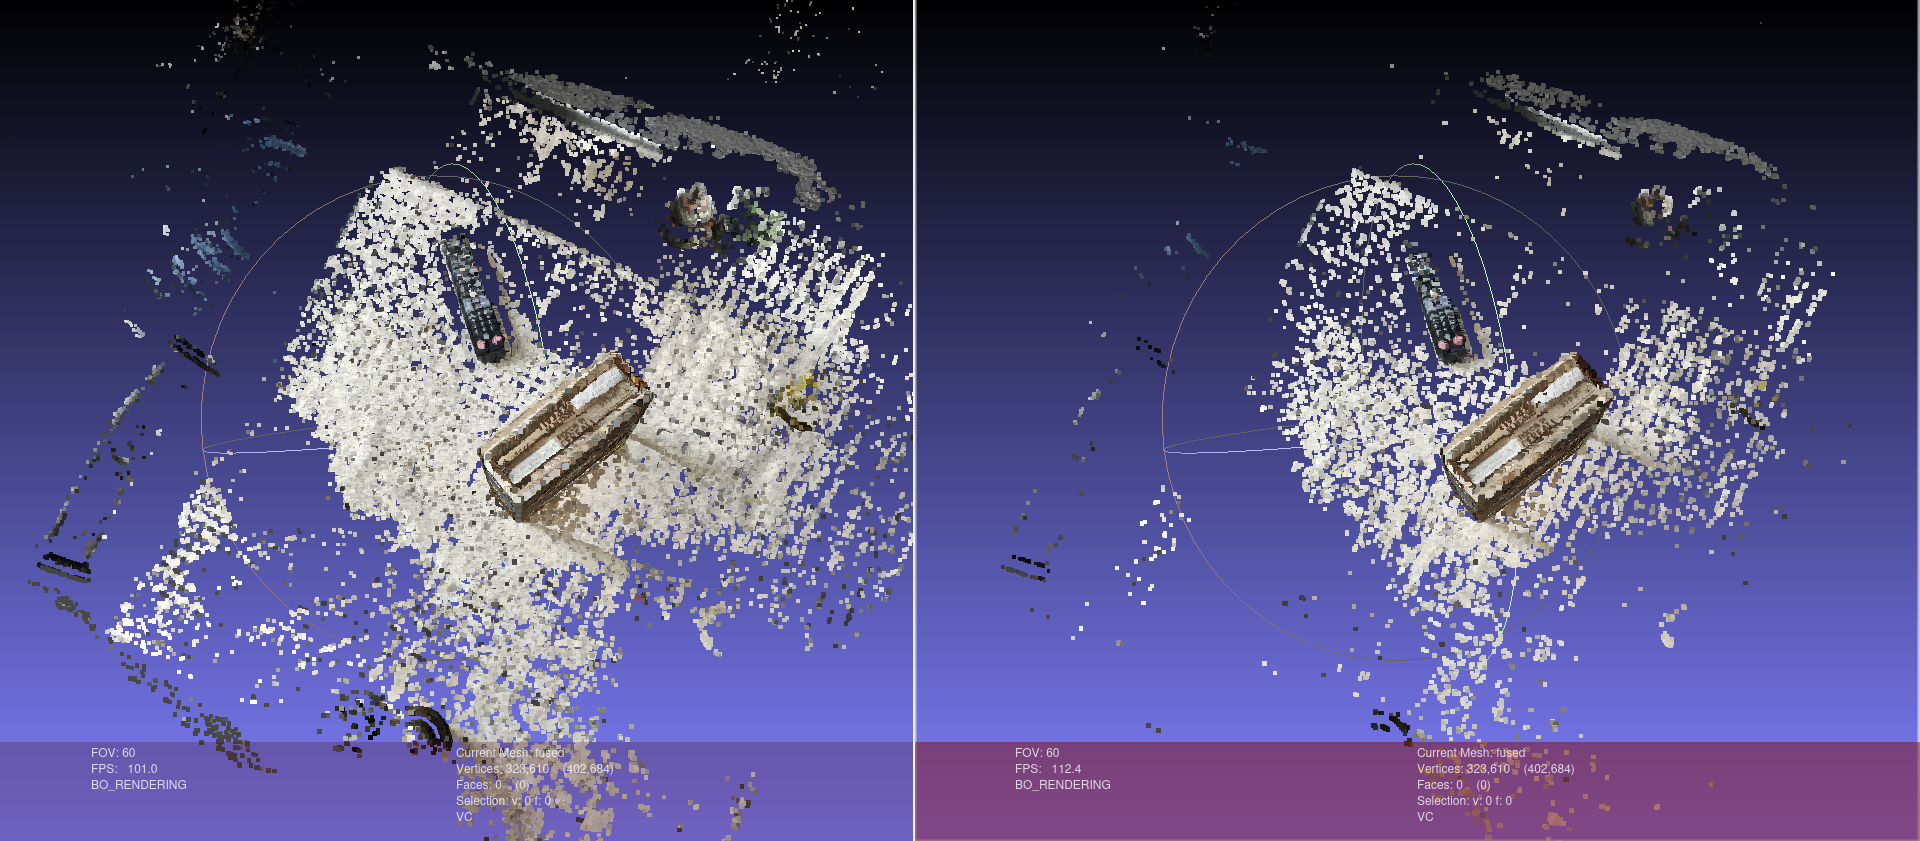
\includegraphics[width=\textwidth,height=\textheight,keepaspectratio]{images/cereal.2.png}
    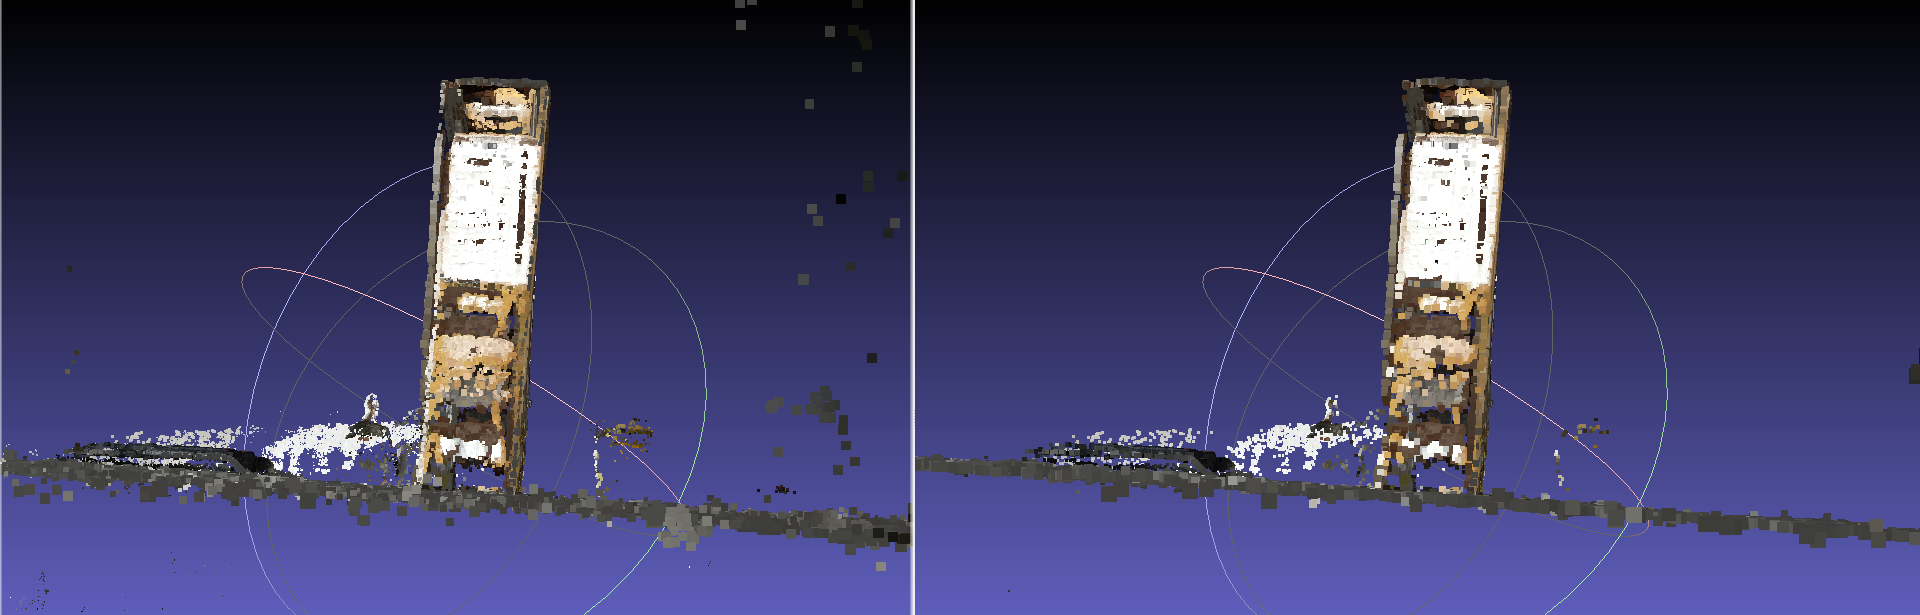
\includegraphics[width=\textwidth,height=\textheight,keepaspectratio]{images/cereal.3.png}
    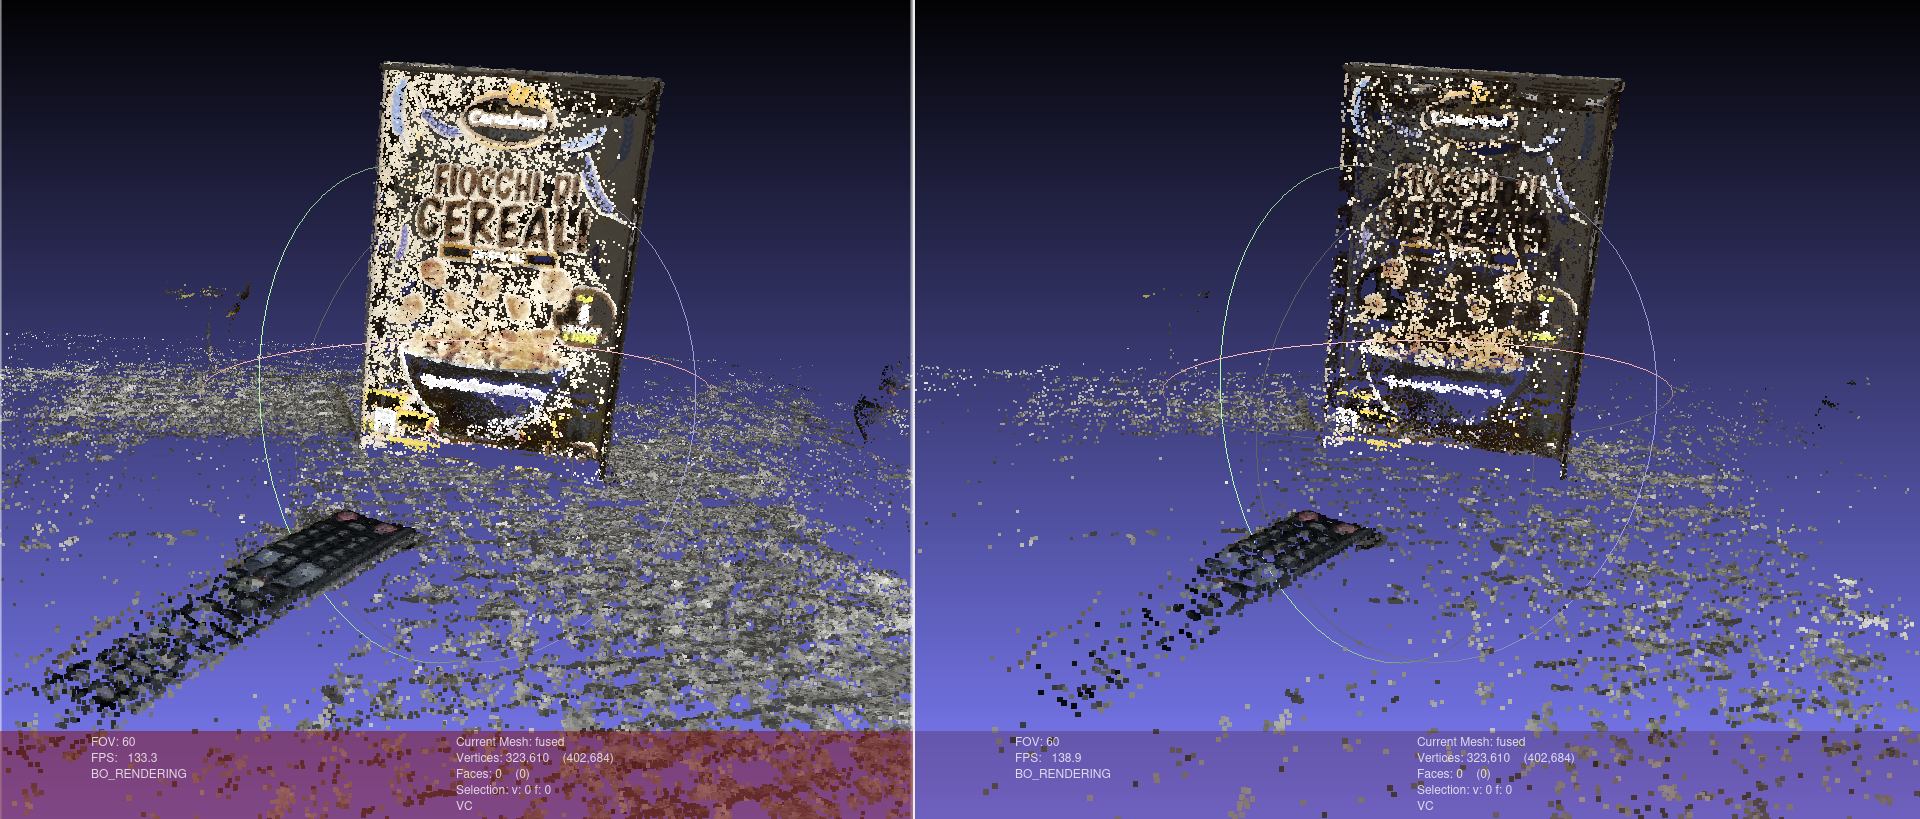
\includegraphics[width=\textwidth,height=\textheight,keepaspectratio]{images/cereal.4.png}
    \caption{Compare The point clouds before(left images) and after refinement(right images)}
    \label{fig:cereal}
    \end{figure}
    \clearpage

    \subsection{Aerial Point Cloud}
    An extensive collection of 3D points is obtained from the city of Padova
    using an airplane. The covered region spans 1600m by 1000m, and the average nearest neighbor distance
    of points is 0.63m. The dataset contains a total of 3,583,803 points, figure \ref{fig:ply_aerial_all}.

    \begin{figure}
    \centering
    \includegraphics[width=\textwidth,height=\textheight,keepaspectratio]{images/experiment/ply_aerial_all}
    \caption{The aerial point cloud from the city of Padova}
    \label{fig:ply_aerial_all}
    \end{figure}

    \section{Point Cloud Registration}
    The objective is to align the ground point cloud with the aerial point cloud. Initially, we attempted
    to register the point cloud using traditional global and local algorithms like FPFH feature matching,
    RANSAC, and ICP. However, due to the significant differences in the nature of the datasets, the results were
    too poor. The aerial point cloud primarily consists of street points and building roofs, as it is captured
    from above. While the ground point cloud contains street points and building walls. Therefore, we had to
    find the common features and simplify the problem. The new pipeline could be described as follows:
    \begin{enumerate}
        \item It was observed that viewing both point clouds from the top point of view, aligned with the z-axis, provides
        valuable information. The first step is to align the point clouds with the z-axis. The aerial
        point cloud is already aligned. The ground point cloud is segmented into planes, and the plane
        with the highest point count is identified as the street plane since it is the common plane among
        all streets and directions and so more points must fall on the ground plane. After that,
        the rotation matrix between the normal vector of the street plane and the (x=0, y=0, z=1) vector
        is computed, and then, the ground point cloud is rotated using the rotation matrix.
        This step determines the rotation around x and y axes, roughly.

        \item From the top point of view, It is seen that the most discriminative feature among the datasets
        is the angles of streets and crossroads. So, the data of vertical walls in ground dataset and roofs
        in aerial dataset has no use. Therefore, both point clouds are sliced along the z-axis with a certain
        threshold and the half related to the streets is remained. In figure \ref{fig:ply_sliced}, the similarity of
        both sliced ground and aerial point clouds are visible.
        \begin{figure}
            \centering
            \begin{subfigure}{0.45\textwidth}
                \centering
                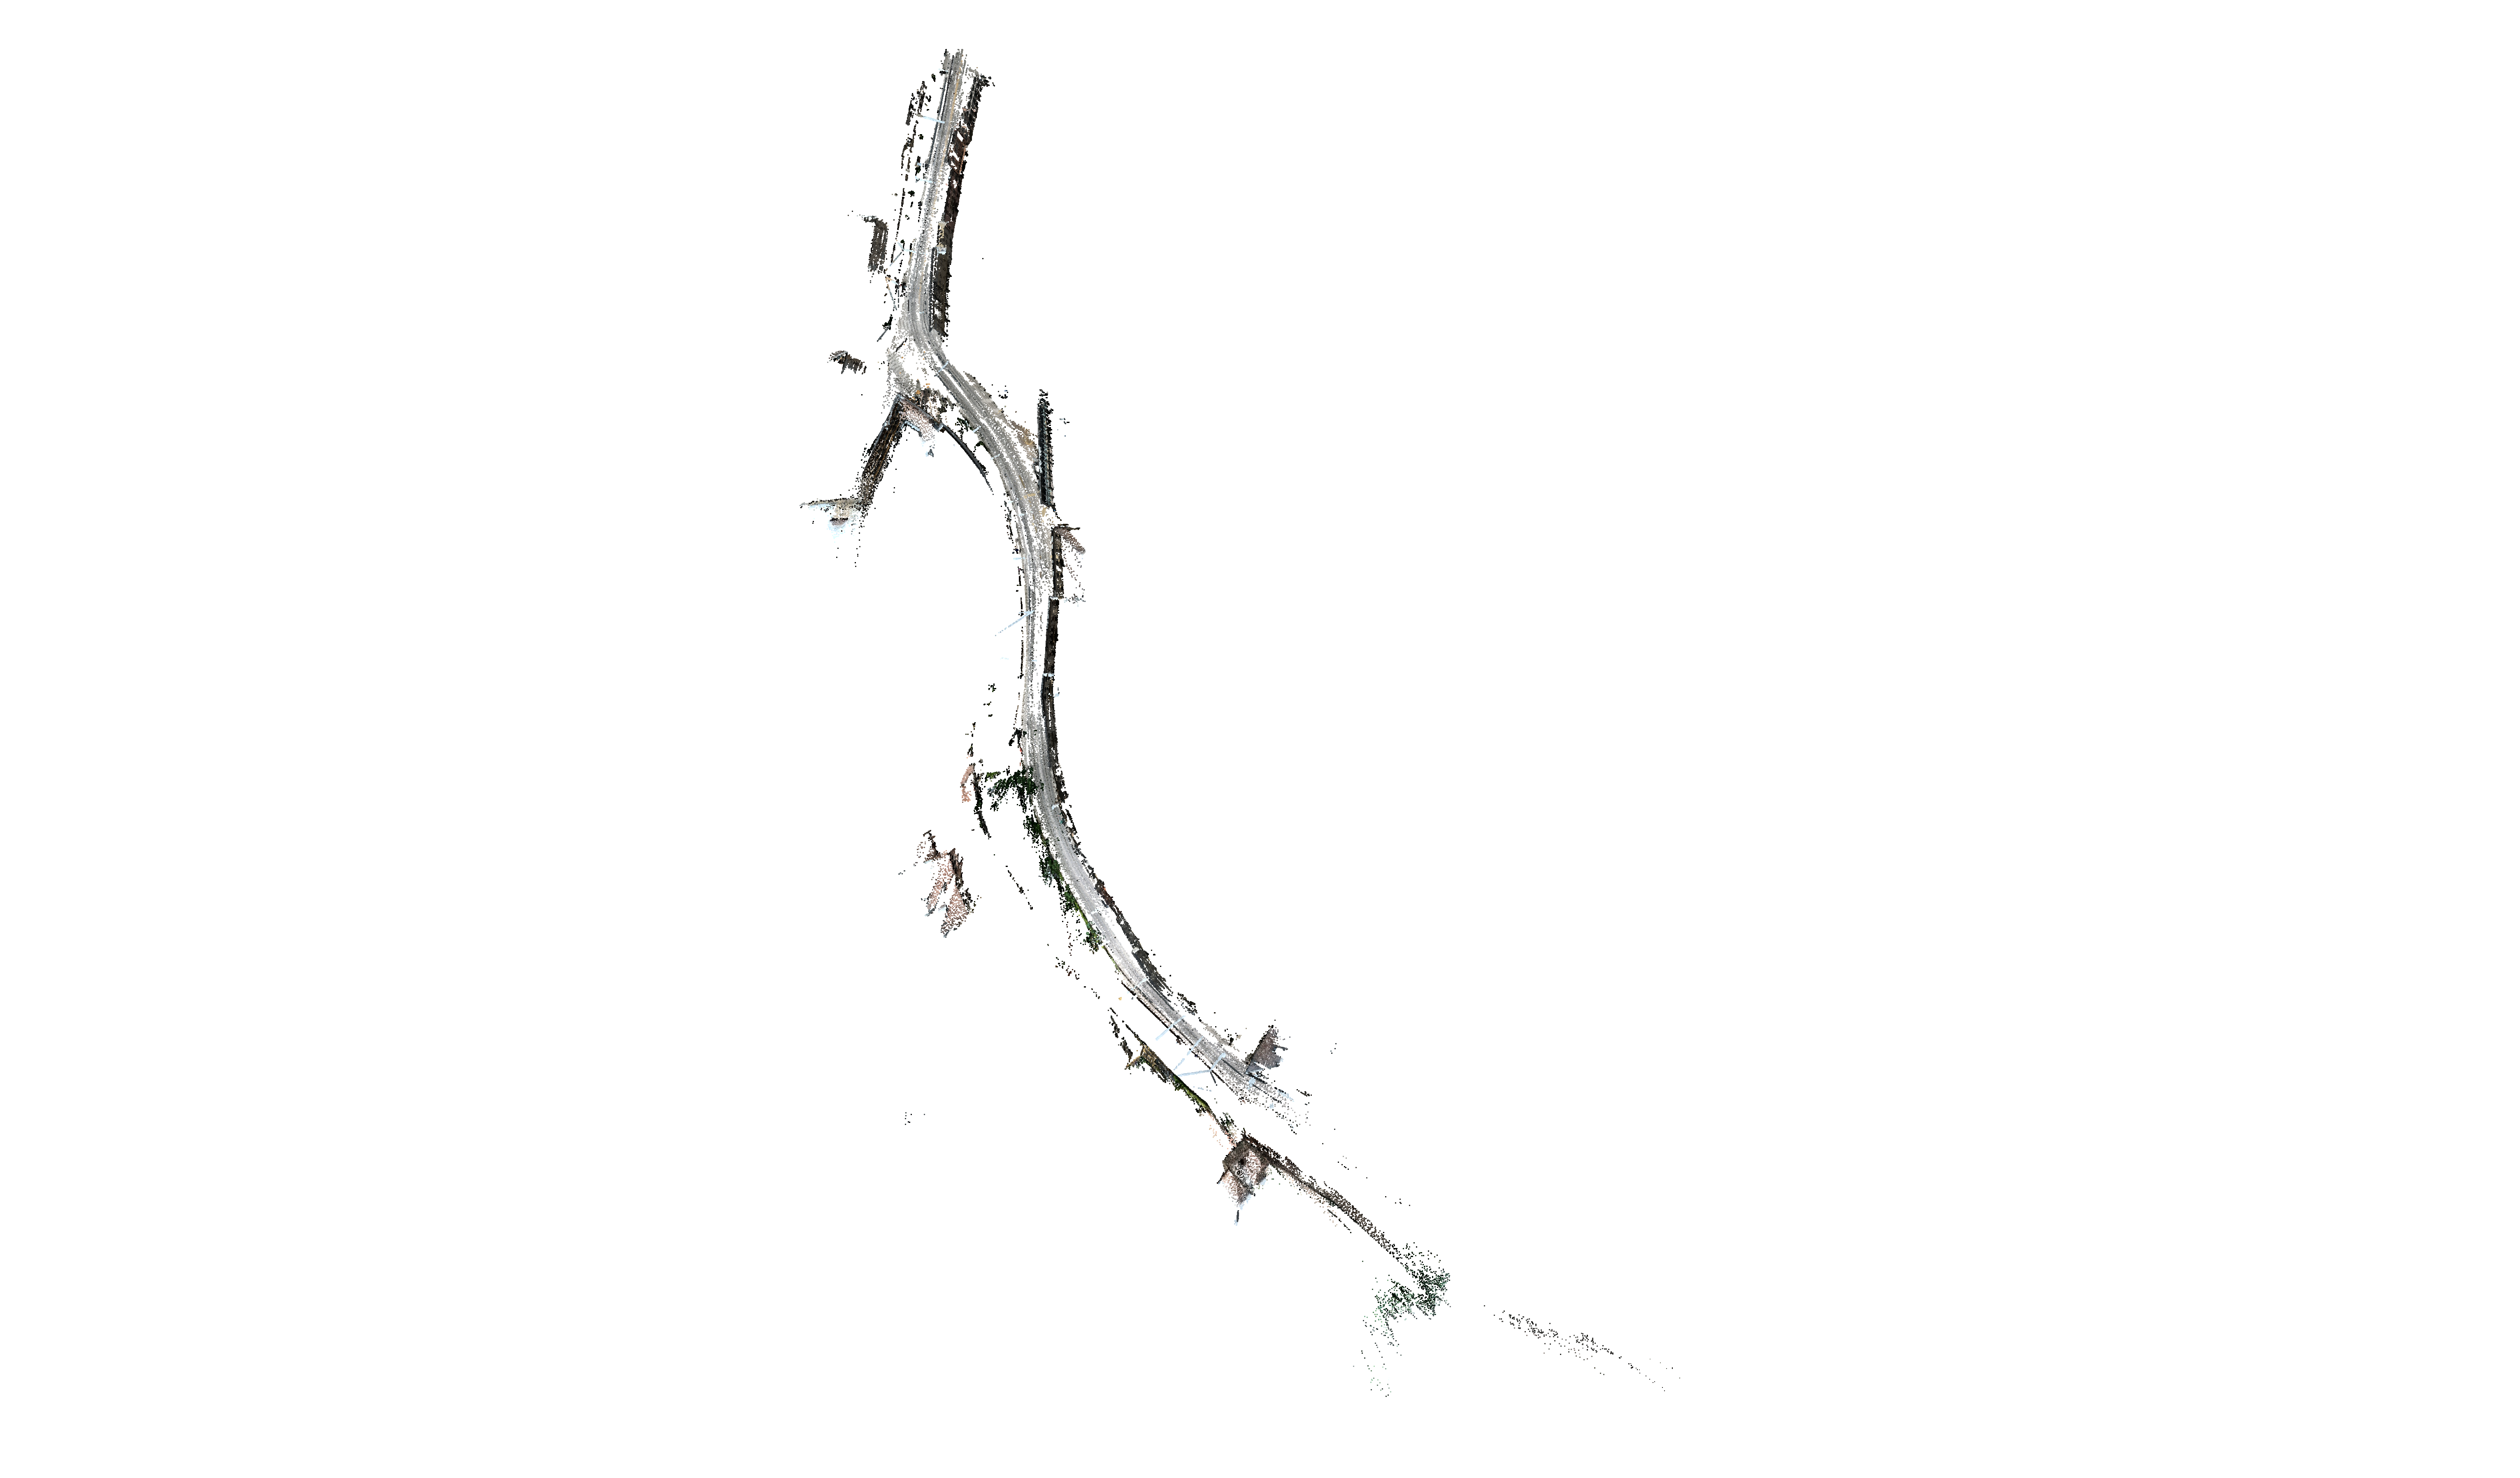
\includegraphics[width=\linewidth]{images/experiment/ply_sliced_ground}
                \caption{Ground Point Cloud}
            \end{subfigure}
            \hfill
            \begin{subfigure}{0.45\textwidth}
                \centering
                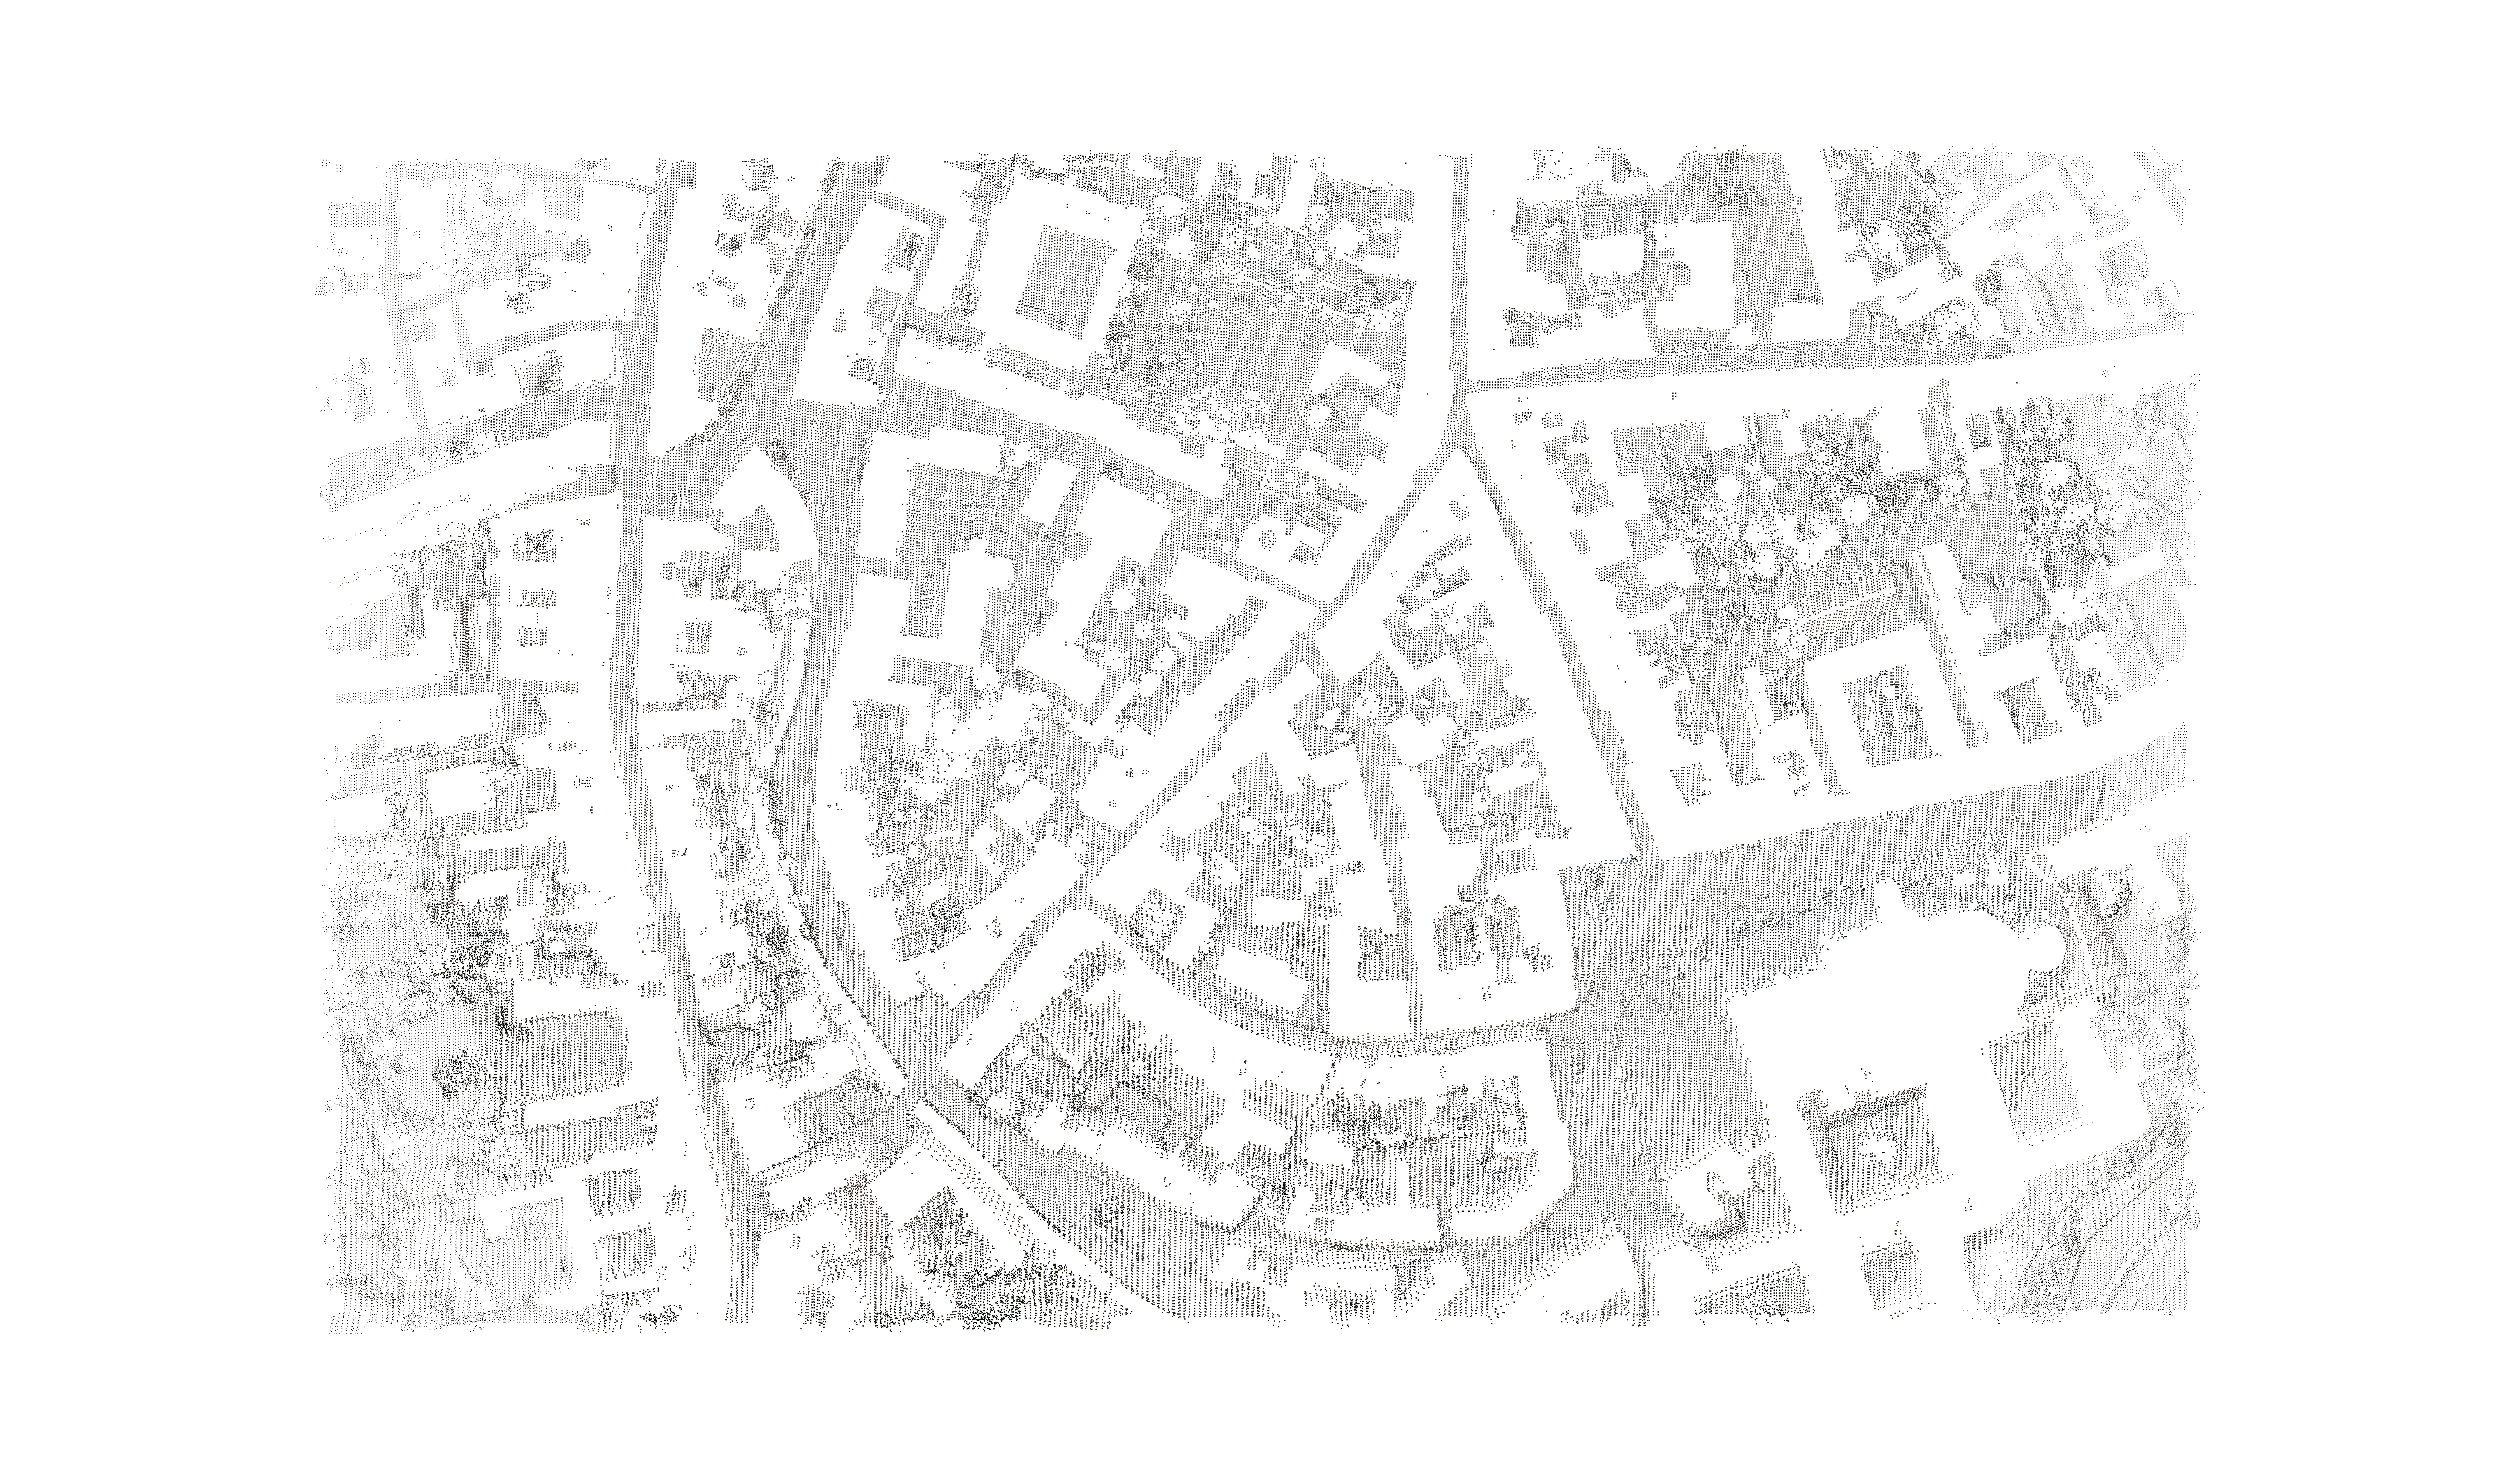
\includegraphics[width=\linewidth]{images/experiment/ply_sliced_aerial}
                \caption{Aerial Point Cloud}
            \end{subfigure}
            \caption{Point clouds sliced from the top viewpoint}
            \label{fig:ply_sliced}
        \end{figure}

        \item Since the generated point clouds has the up-to-scale problem, it is needed to normalize the
        coordinate values across all datasets. This step does not scale the ground point clouds to the actual size
        in aerial point cloud. However, it ensures that the average minimum distance between the points is the same
        among all of the generated point clouds.
        Each point cloud is scaled by the factor of 1 divided by the current average of the minimum distance to the nearest point.

        \item A 2D binary map is generated for each point cloud considering only x and y coordinates of all 3D points.
        The dimensions of the map are determined by calculating the difference between the maximum and minimum x and y
        coordinates of all points and dividing it by a predefined resolution value. Each cell in the map is assigned
        a value of 1 if at least one point's x and y coordinates fall within that cell, indicating the presence of
        points in that area. Conversely, if there are no points corresponding to the respective x and y coordinates,
        the cell is marked as 0. In the binary grid map for Ground Point Cloud, considering that each point cloud is
        generated from a sequence of video frames, the camera pose of the middle frame is regarded as the ground truth
        center position for the entire dataset. To evaluate the registration method's robustness and generalization,
        3 aerial point clouds are considered for each ground dataset. These aerial point clouds share the same center
        as the aforementioned ground point cloud, but they differ in distance from the center. They are categorized
        as "easy," "medium," and "hard" with distances of 100, 150, and 200 meters from each direction, respectively.
        The binary grid map is generated for these aerial point clouds using the same logic as the binary grid map
        created for the ground point clouds.

        \item To localize the ground grid map within the aerial grid maps, various methods were explored, including
        2D feature matching, crossroad detection based on point counting, and training convolutional neural networks,
        etc. Among these approaches, template matching has the best results. The template matching process involves
        comparing a small template image, which represents the desired pattern (in this case, the ground grid map),
        with different regions of the target image (the aerial grid map), and identify the region that has the highest
        similarity with the template. This is achieved by moving a window across the target
        image and comparing the template with each window. We extended the algorithm to compare also different
        scales and rotations of the template image. The template is rotated up to 360 degrees with an interval of 10 degrees and
        scaled from 10\% to 200\% of its initial size, increasing 10 percent per each attempt.

    \end{enumerate}

    \section{Final algorithm}
    The whole pipeline can be summarized as follows:
    \begin{enumerate}
        \item Take the video of the streets and extract the frames
        \item Run sparse SfM algorithm
        \item Refine the sparse point cloud and camera poses using Pixel Perfect algorithm
        \item Generate a dense point cloud from the refined data
        \item Align the point cloud along the z-axis.
        \item Scale and Slice the ground point cloud, and keep the points with z coordinate less than a threshold,
        in our case, the threshold is 20\% of the minimum z-coordinate
        \item Generate the binary grid map
        \item Slice Aerial point cloud along the z-axis with a certain threshold, in our case, the threshold is 20\%
        of the minimum of z coordinate of all points
        \item Generate Binary grid map for Aerial point cloud
        \item Run Template Matching algorithm to localize the ground grid map inside the aerial grind map
    \end{enumerate}


\end{document}